% Options for packages loaded elsewhere
\PassOptionsToPackage{unicode}{hyperref}
\PassOptionsToPackage{hyphens}{url}
%
\documentclass[
  english,
  man,floatsintext]{apa7}
\usepackage{lmodern}
\usepackage{amsmath}
\usepackage{ifxetex,ifluatex}
\ifnum 0\ifxetex 1\fi\ifluatex 1\fi=0 % if pdftex
  \usepackage[T1]{fontenc}
  \usepackage[utf8]{inputenc}
  \usepackage{textcomp} % provide euro and other symbols
  \usepackage{amssymb}
\else % if luatex or xetex
  \usepackage{unicode-math}
  \defaultfontfeatures{Scale=MatchLowercase}
  \defaultfontfeatures[\rmfamily]{Ligatures=TeX,Scale=1}
\fi
% Use upquote if available, for straight quotes in verbatim environments
\IfFileExists{upquote.sty}{\usepackage{upquote}}{}
\IfFileExists{microtype.sty}{% use microtype if available
  \usepackage[]{microtype}
  \UseMicrotypeSet[protrusion]{basicmath} % disable protrusion for tt fonts
}{}
\makeatletter
\@ifundefined{KOMAClassName}{% if non-KOMA class
  \IfFileExists{parskip.sty}{%
    \usepackage{parskip}
  }{% else
    \setlength{\parindent}{0pt}
    \setlength{\parskip}{6pt plus 2pt minus 1pt}}
}{% if KOMA class
  \KOMAoptions{parskip=half}}
\makeatother
\usepackage{xcolor}
\IfFileExists{xurl.sty}{\usepackage{xurl}}{} % add URL line breaks if available
\IfFileExists{bookmark.sty}{\usepackage{bookmark}}{\usepackage{hyperref}}
\hypersetup{
  pdftitle={Effects of self-compassion on post-traumatic growth and PTSD},
  pdfauthor={Corrado Caudek1, Celeste Berti1, Claudio Sica2, \& Ilaria Colpizzi1},
  pdflang={en-EN},
  pdfkeywords={keywords},
  hidelinks,
  pdfcreator={LaTeX via pandoc}}
\urlstyle{same} % disable monospaced font for URLs
\usepackage{graphicx}
\makeatletter
\def\maxwidth{\ifdim\Gin@nat@width>\linewidth\linewidth\else\Gin@nat@width\fi}
\def\maxheight{\ifdim\Gin@nat@height>\textheight\textheight\else\Gin@nat@height\fi}
\makeatother
% Scale images if necessary, so that they will not overflow the page
% margins by default, and it is still possible to overwrite the defaults
% using explicit options in \includegraphics[width, height, ...]{}
\setkeys{Gin}{width=\maxwidth,height=\maxheight,keepaspectratio}
% Set default figure placement to htbp
\makeatletter
\def\fps@figure{htbp}
\makeatother
\setlength{\emergencystretch}{3em} % prevent overfull lines
\providecommand{\tightlist}{%
  \setlength{\itemsep}{0pt}\setlength{\parskip}{0pt}}
\setcounter{secnumdepth}{-\maxdimen} % remove section numbering
% Make \paragraph and \subparagraph free-standing
\ifx\paragraph\undefined\else
  \let\oldparagraph\paragraph
  \renewcommand{\paragraph}[1]{\oldparagraph{#1}\mbox{}}
\fi
\ifx\subparagraph\undefined\else
  \let\oldsubparagraph\subparagraph
  \renewcommand{\subparagraph}[1]{\oldsubparagraph{#1}\mbox{}}
\fi
% Manuscript styling
\usepackage{upgreek}
\captionsetup{font=singlespacing,justification=justified}

% Table formatting
\usepackage{longtable}
\usepackage{lscape}
% \usepackage[counterclockwise]{rotating}   % Landscape page setup for large tables
\usepackage{multirow}		% Table styling
\usepackage{tabularx}		% Control Column width
\usepackage[flushleft]{threeparttable}	% Allows for three part tables with a specified notes section
\usepackage{threeparttablex}            % Lets threeparttable work with longtable

% Create new environments so endfloat can handle them
% \newenvironment{ltable}
%   {\begin{landscape}\begin{center}\begin{threeparttable}}
%   {\end{threeparttable}\end{center}\end{landscape}}
\newenvironment{lltable}{\begin{landscape}\begin{center}\begin{ThreePartTable}}{\end{ThreePartTable}\end{center}\end{landscape}}

% Enables adjusting longtable caption width to table width
% Solution found at http://golatex.de/longtable-mit-caption-so-breit-wie-die-tabelle-t15767.html
\makeatletter
\newcommand\LastLTentrywidth{1em}
\newlength\longtablewidth
\setlength{\longtablewidth}{1in}
\newcommand{\getlongtablewidth}{\begingroup \ifcsname LT@\roman{LT@tables}\endcsname \global\longtablewidth=0pt \renewcommand{\LT@entry}[2]{\global\advance\longtablewidth by ##2\relax\gdef\LastLTentrywidth{##2}}\@nameuse{LT@\roman{LT@tables}} \fi \endgroup}

% \setlength{\parindent}{0.5in}
% \setlength{\parskip}{0pt plus 0pt minus 0pt}

% \usepackage{etoolbox}
\makeatletter
\patchcmd{\HyOrg@maketitle}
  {\section{\normalfont\normalsize\abstractname}}
  {\section*{\normalfont\normalsize\abstractname}}
  {}{\typeout{Failed to patch abstract.}}
\patchcmd{\HyOrg@maketitle}
  {\section{\protect\normalfont{\@title}}}
  {\section*{\protect\normalfont{\@title}}}
  {}{\typeout{Failed to patch title.}}
\makeatother
\shorttitle{Construct validity of SCS}
\keywords{keywords\newline\indent Word count: 4466}
\usepackage{lineno}

\linenumbers
\usepackage{csquotes}
\usepackage{rotating}
\DeclareDelayedFloatFlavor{sidewaysfigure}{figure}
\DeclareDelayedFloatFlavor{sidewaystable}{table}
\usepackage{pdflscape}
\DeclareDelayedFloatFlavor{landscape}{table}
\raggedbottom
\usepackage{xcolor,makecell,array}
\usepackage{graphicx}
\usepackage{placeins}
\setlength{\parskip}{0pt plus 0pt minus 0pt}
\usepackage{multirow}
\usepackage{setspace}
\usepackage{booktabs}
\usepackage{tabularx}
\usepackage{caption}
\usepackage{color, colortbl}
\ifxetex
  % Load polyglossia as late as possible: uses bidi with RTL langages (e.g. Hebrew, Arabic)
  \usepackage{polyglossia}
  \setmainlanguage[]{english}
\else
  \usepackage[shorthands=off,main=english]{babel}
\fi
\ifluatex
  \usepackage{selnolig}  % disable illegal ligatures
\fi
\newlength{\cslhangindent}
\setlength{\cslhangindent}{1.5em}
\newlength{\csllabelwidth}
\setlength{\csllabelwidth}{3em}
\newenvironment{CSLReferences}[2] % #1 hanging-ident, #2 entry spacing
 {% don't indent paragraphs
  \setlength{\parindent}{0pt}
  % turn on hanging indent if param 1 is 1
  \ifodd #1 \everypar{\setlength{\hangindent}{\cslhangindent}}\ignorespaces\fi
  % set entry spacing
  \ifnum #2 > 0
  \setlength{\parskip}{#2\baselineskip}
  \fi
 }%
 {}
\usepackage{calc}
\newcommand{\CSLBlock}[1]{#1\hfill\break}
\newcommand{\CSLLeftMargin}[1]{\parbox[t]{\csllabelwidth}{#1}}
\newcommand{\CSLRightInline}[1]{\parbox[t]{\linewidth - \csllabelwidth}{#1}\break}
\newcommand{\CSLIndent}[1]{\hspace{\cslhangindent}#1}

\title{Effects of self-compassion on post-traumatic growth and PTSD}
\author{Corrado Caudek\textsuperscript{1}, Celeste Berti\textsuperscript{1}, Claudio Sica\textsuperscript{2}, \& Ilaria Colpizzi\textsuperscript{1}}
\date{}


\authornote{

Add complete departmental affiliations for each author here. Each new line herein must be indented, like this line.
Enter author note here.

Correspondence concerning this article should be addressed to Corrado Caudek, NEUROFARBA Department, Psychology Section, University of Firenze, Italy. E-mail: \href{mailto:ccaudek@unifi.it}{\nolinkurl{ccaudek@unifi.it}}

}

\affiliation{\vspace{0.5cm}\textsuperscript{1} NEUROFARBA Department, Psychology Section, University of Florence, Italy\\\textsuperscript{2} Health Sciences Department, Psychology Section, University of Florence, Italy}

\abstract{
One or two sentences providing a \textbf{basic introduction} to the field, comprehensible to a scientist in any discipline.

Two to three sentences of \textbf{more detailed background}, comprehensible to scientists in related disciplines.

One sentence clearly stating the \textbf{general problem} being addressed by this particular study.

One sentence summarizing the main result (with the words ``\textbf{here we show}'' or their equivalent).

Two or three sentences explaining what the \textbf{main result} reveals in direct comparison to what was thought to be the case previously, or how the main result adds to previous knowledge.

One or two sentences to put the results into a more \textbf{general context}.

Two or three sentences to provide a \textbf{broader perspective}, readily comprehensible to a scientist in any discipline.
}



\begin{document}
\maketitle

\hypertarget{introduction}{%
\section{Introduction}\label{introduction}}

Self-compassion is a construct derived from the Buddhist tradition and has been conceptualized by Neff (2003b) as motivation to adopt a compassionate mindset towards themselves in order to prevent suffering of self and others.
Self-compassion (SC) has been proposed as a protective factor against psychopathology, including PTSD, and as a factor promoting PTG (ref).

The SC construct is typically assessed with the Self-Compassion Scale (SCS), a 26 item self-report scale (Neff, 2003b).
The SCS items span six dimensions of the construct.
Three sub-sets of items are indicators of compassionate self-responding: (a) being kind and understanding toward one's fallibility, (b) acknowledging that personal failures and pain are something that everyone experiences, and (c) having a mindful awareness of one's painful thoughts and feelings.
The remaining three sub-sets of items are indicators of the negation of uncompassionate self-responding: (a) being critical and not understanding toward personal shortcomings, (b) having the tendency of isolating from others, and (c) avoiding one's painful thoughts and feelings or overidentifying with them.
The SCS total score is given by the sum of the self-responding on the compassionate items and the reversely scored uncompassionate items.

The construct of SC and the SCS has been extremely popular in the recent psychological literature (for a recent review, see Muris \& Otgaar, 2020).
A measure of such success is provided, for example, by a search of the literature conducted on December 18, 2020 using ``self compassion'' in Topic as a search term, which yielded 2,380 results.
However, the growing success of the SCS has not been unchallenged and questions have been raised about the validity of this scale (Kandler et al., 2017; Muris, 2016; Muris et al., 2016, 2019; Muris \& Petrocchi, 2017).

Muris and Otgaar (2020), for example, has pointed to the fact that the common practice of considering the construct measured by the SCS as a unitary construct is problematic:

\begin{quote}
We argue that this criticism is far from trivial and seriously undermines the scientific foundation of the self-compassion concept (p.~1473).
\end{quote}

In several papers, Muris and collaborators have pointed out the fact that researchers tend to treat the SC construct as a ``pure protective factor,'' rather than to present a more nuanced picture of SC (e.g., Gu et al., 2020; Montero-Marin et al., 2018; Seppälä et al., 2017; Strauss et al., 2016) and, as a consequence of this, the data of the SCS are usually summarized in terms of the SCS total score.
But the use of the total score is problematic for several reasons.
For the present purposes, it is important to focus on the following two criticisms.

\begin{enumerate}
\def\labelenumi{\arabic{enumi}.}
\tightlist
\item
  The use of the SCS total score tend to inflate the link with psychopathology. According to Muris et al. (2018), in fact, the relations that have been found between the SCS total scores and other psychological constructs mainly depend on the uncompassionate component of the SCS. But the uncompassionate component of the SCS is strongly associated with (reversed) Negative Affect and, once the negative component of SC is removed, the added value of positive SC is marginal.
\end{enumerate}

\begin{enumerate}
\def\labelenumi{\arabic{enumi}.}
\setcounter{enumi}{1}
\tightlist
\item
  It is not clear what, if anything, is added by the compassionate component of the SCS to the nomological network in which SC is situated. Kandler et al. (2017) have taken the extreme stance of arguing that the SC construct is redundant because it overlaps with with the personality trait of Neuroticism: Once Neuroticism is controlled, there is no evidence of a specific contribution of SC.
\end{enumerate}

This debate has receiving considerable attention in the recent literature on SC, because the questions that have been raised are relevant for therapeutic interventions.
In fact, it is of interest to understand whether the association between the treatment effects and the compassionate component of SC may be obscured by the common use of the SCS total score (Wadsworth et al., 2018).

In summary, the criticisms that have been directed towards the use of the SCS total score as a proxy for the SC construct point to the necessity of (1) distinguishing the compassionate self-responding from the uncompassionate component of the SCS, (2) evaluating the relative contribution of each of these two components, and (3) establishing whether the the compassionate self-responding has incremental value above and beyond other psychological factors currently examined in therapeutic settings, in primis the personality trait of Neuroticism.

\begin{center}\rule{0.5\linewidth}{0.5pt}\end{center}

As a consequence, it has been asked whether the construct of SC (as measured by the SCS) is useful (in that it adds something new) or whether it is redundant, as it can be replaced with the personality trait of neuroticism (Kandler et al., 2017).
Specifically, given that the total score of the SCS is given by the sum of the indicators of the compassionate and uncompassionate components of the SCS, the question has been raised about the relative contribution of the compassionate components of SC to the total score.

One limit of these studies, however, is that they have often been performed in student populations, that is, in samples in which, supposedly, PTSD and PTG are only present in mild forms.
The purpose of the present study is to evaluate the hypotheses of Muris et al. (2019) and of Geiger et al. (2018) in a sample of rescue workers.

Rescue workers are a population at risk for high levels of burnout and compassion fatigue.
???

Questions:

\begin{itemize}
\item
  \textbf{HP1}: Is the construct of self-compassion (SC) necessary?
  It has been proposed that the effects of self-compassion can be due only to the negative component of SC, whereas the positive component of SC has no effect.
  If this were true, then there would be no need of the construct of SC, given that the negative component of SC reduces to negative affect (ref).
  To answer this question is necessary to show that the positive component of SC has an effect on other psychological constructs, beyond that of the negative component of SC.
\item
  \textbf{HP2}: It has been argued that SC reduces to nevroticism.
  Again, it this were true, then we would not need the separate construct of SC.
  In order to test this hypothesis (ref) it would be necessary to show that both components of SC provide an added value in a nomological network which includes the construct of nevroticism.
\end{itemize}

In the present study we tested these two hypotheses by comparing different SEM models including the folloging constructs\ldots{}

PTSS and PTG emerge only in individuals subjected to high load of psychological stress.
For this reason, we examined a large sample of rescue workers.

\hypertarget{methods}{%
\section{Methods}\label{methods}}

\hypertarget{participants}{%
\subsection{Participants}\label{participants}}

\hypertarget{material}{%
\subsection{Material}\label{material}}

Specific questions for ambulance personnel were developed to investigate the role that the respondent usually covered (such as driver, team leader, rescuer, etc.), number of weekly shifts, and number of psychological support meeting (such as debriefing and defusing) every participants have requested during the last two weeks and their careers (e.g.~``How often are you on ambulance duty?'' and ``Do you usually take shift with the same team?'').
Moreover, the researchers asked participants to tell about a traumatic event occurs during their careers, which they felt seriously affected by (e.g.~``Would you mind to briefly describe a traumatic event you have experienced during your career?'').

Personality traits were assessed using the \emph{NEO-Five Factor Inventory} (NEO-FFI-60; Costa \& McCrae, 1992; Italian version by Caprara et al., 2001), based upon the Five Factors Model (FFM) of personality traits (McCrae \& Costa, 1987).
The NEO-FFI-60 is a 60 items self-report questionnaire that allows the assessment of five broad personality domains: Neuroticism (N), Extraversion (E), Openness to Experience (O), Agreeableness (A), and Conscientiousness (C).
The respondent is asked to rate the items on 5-point Likert scale ranging from 0 (Strongly disagree) to 4 (Strongly agree).
NEO-FFI showed good internal consistency, Cronbach's alpha ranging from .68 (A) to .89 (N).

The coping strategies were investigated using the Italian version of the \emph{Coping Orientation to Problem Experienced Inventory} (COPE, Carver et al., 1989; Sica et al., 2008).
COPE is a self-report questionnaire composed by 60 items used to assess a wide range of coping strategies gathered in 15 scales: 1) active coping, 2) planning, 3) seeking instrumental social support, 4) seeking emotional social support, 5) suppression of competing activities, 6) turning to religion, 7) positive reinterpretation and growth, 8) restraint coping, 9) acceptance, 10) focus on and venting of emotions, 11) denial, 12) mental disengagement, 13) behavioral disengagement, 14) alcohol/drug use, and 15) humor.
The scales were grouped in the following dimension: Problem focused, Avoidant coping, Social support, Emotion focused and Religion.
The items are rated on a 4-point Likert scale ranging from 1 (I don't usually do that) to 4 (I usually do that).
Internal consistency (Chronbach's \(\alpha\)) ranging from \(\alpha\) = .70 to \(\alpha\) = .91.

The \emph{Post-Traumatic Growth Inventory} (PTGI; Tedeschi \& Calhoun, 1996; Italian version by Prati \& Pietrantoni, 2006) is a 21 item self-report measure.
PTGI evaluates the growth following one or more stressful or traumatic events in one's life.
The item score ranging on a 7-point Likert scale, from 0 (No change) to 6 (Very important change).
The PTGI comprises five subscales: Relation with others, New possibilities, Personal strength, Appreciation of life, and Spiritual changes.
The Incident of Event Scale - revised (IES-R; Horowitz et al., 1979; Weiss \& Marmar, 1997; Weiss, 2004) is widely used to assess the symptomatology of the Post-Traumatic Stress Disorder in rescue workers.
IES-R is used to investigate the three symptoms of PTSD: Intrusion, Hypervigilance, and Avoidance.
The score ranging on a 5-point Likert scale from 0 (Not at all) to 4 (Extremely).
Each subscale showed high internal consistency (Chronbach's \(\alpha\)), intrusion = 0.87 to 0.94, avoidance = 0.84 to 0.97, hyperarousal = 0.79 to 0.91.

Self-compassion was measured using the 26 items of the \emph{Self-Compassion Scale} (SCS; Neff, 2003; Italian version by Veneziani et al., 2017).
This self-report questionnaire is composed by two subscales which are divided in three component themselves: Self-Kindness, Common Humanity, and Mindfulness identified the positive subscale, while Self-Judgement, Isolation, and Overidentification the negative subscale.
SCS score ranging on a 5-point Likert scale from 1 (Almost always) to 5 (Almost never).
High scores of self-compassion reflect an ability to be kind and understanding toward oneself, even in difficult times.
Internal consistency for unidimensional Self-Compassion was found of 0.92 (Neff, 2003a).

TODO: reliability of the SCS with the present sample

For the present sample, consistently with Neff et al. (2019), reliability was computed by examining a bi-factor model in which each loaded on its corresponding factor, but also on an overarching factor.

Multi-dimensional Scale of Perceived Social Support (MSPSS; Zimet et al., 1988; Italian version by Prezza \& Pacilli, 2002) was used to assess how participants perceived social support.
MSPSS is a 12 items self-report questionnaire, and respondent was asked to rate their experience of perceived support from Family, Friends, and Significant Others.
MSPSS showed an internal consistency between 0.80 and 0.95 (Ozdemir, 2019).

\hypertarget{procedure}{%
\subsection{Procedure}\label{procedure}}

\hypertarget{data-analysis}{%
\subsection{Data analysis}\label{data-analysis}}

TODO

\hypertarget{results}{%
\section{Results}\label{results}}

\hypertarget{preliminary-analysis-and-descriptive-statistics}{%
\subsection{Preliminary Analysis and Descriptive Statistics}\label{preliminary-analysis-and-descriptive-statistics}}

The goodness‐of‐fit was evaluated according to the Comparative Fit Index (CFI), Tucker-Lewis Index (TLI), Root Mean Square Error Approximation (RMSEA), and Standardized Root Mean Square Residual (SRMR).
The following cut-off criteria were used: RMSEA and SRMR near or less than 0.08, and CFI and TLI near or greater than 0.90 (Little, 2013).
All models were tested using Mplus version 8.5 (Muthén \& Muthén, 2017) using all available data.
A weighted least squares mean- and variance-adjusted estimator (WLSMV) was used to assess each latent construct, as it is more adequate than maximum-likelihood for ordered-categorical items with five or less response options (e.g., Bandalos, 2014).

We started with the unidimensional CFA model, which clearly proved to be inadequate, CFI = 0.61, TLI = 0.58, RMSEA = 0.18 {[}90\% CI 0.18-0.19{]}, SRMR = 0.16.
We then considered all the factor structures for the SCS that had been discussed by Neff et al. (2019). The list of the examined models, together with their fit indices, is provide below:

\begin{itemize}
\item
  a two-factor CFA for the positive and the negative components of SC, CFI = 0.83, TLI = 0.82, RMSEA = 0.12 {[}90\% CI 0.12-0.12{]}, SRMR = 0.10;
\item
  a two-factor ESEM, CFI = 0.85, TLI = 0.82, RMSEA = 0.12 {[}90\% CI 0.12-0.12{]}, SRMR = 0.06;
\item
  a six-factor CFA, CFI = 0.90, TLI = 0.88, RMSEA = 0.10 {[}90\% CI 0.09-0.10{]}, SRMR = 0.07;
\item
  a six-factor ESEM, CFI = 0.98, TLI = 0.96, RMSEA = 0.05 {[}90\% CI 0.05-0.06{]}, SRMR = 0.02;
\item
  a bifactor-CFA (1 G- and 6 S-factors), CFI = 0.76, TLI = 0.71, RMSEA = 0.15 {[}90\% CI 0.15-0.16{]}, SRMR = 0.12;
\item
  a bifactor-ESEM (1 G- and 6 S-factors), CFI = 0.98, TLI = 0.96, RMSEA = 0.05 {[}90\% CI 0.05-0.06{]}, SRMR = 0.02;
\item
  a two-bifactor (two-tier) CFA model (2 G- and 6 S-factors), CFI = 0.90, TLI = 0.88, RMSEA = 0.10 {[}90\% CI 0.10-0.10{]}, SRMR = 0.08;
\item
  a two-bifactor (two-tier) ESEM model (2 G- and 6 S-factors), CFI = 0.99, TLI = 0.98, RMSEA = 0.04 {[}90\% CI 0.04-0.05{]}, SRMR = 0.01.
\end{itemize}

For the two-factor CFA for the CS and RUS of SC, the correlation between the factors was -0.28.
For the two-factor ESEM, the correlation between the factors was -0.21.
For the 6-factor CFA, the correlations between factors ranged between -0.44 and 0.95.
For the 6-factor ESEM, the correlations between factors ranged between -0.36 and 0.58.
For the two-bifactor (two-tier) CFA model (2 G- and 6 S-factors), the correlation between the CS and RUS factors is -0.34.
For the two-bifactor (two-tier) ESEM model (2 G- and 6 S-factors), the correlation between the CS and RUS factors is -0.55.

The present results replicate what reported by Neff et al. (2019) and indicate that the bifactor ESEM models (\emph{i.e.}, Models 4b and 5b in the original paper) provides the best description of the factor structure of the SC scale. In our data, both a bifactor-ESEM (1 G- and 6 S-factors) and a two-bifactor (two-tier) ESEM model (2 G- and 6 S-factors) provided an excellent adaptation to the data. Specifically, the two-bifactor (two-tier) ESEM model included 6 uncorrelated factors (self-kindness, reduced self-judgment, common humanity, reduced isolation, mindfulness, and reduced over-identification) and two correlated CS (loading on the self-kindness, common humanity, and mindfulness items) and RUS (loading on the reduced self-judgment, reduced isolation, and reduced over-identification items) factors and showed a marginally better fit than the one bifactor-ESEM (1 G- and 6 S-factors) model. What is crucial is that the models discussed by Neff et al. (2019), and here reproduced, include distinct factors which correspond to the six dimensions of the SCS: self-kindness, reduced self-judgment, common humanity, reduced isolation, mindfulness, and reduced over-identification. Also in the present sample, these two models, which are closer to the view that self-compassion is comprised of six components that interact as a global system (Neff, 2003a), provide the best fit to the data.

In the following, we present three further factor models that are not discussed by Neff et al. (2019). A description of the models together with their fit indices is proveded below.

To start, we considered a bifactor two-factor ESEM, with correlated SC and RUS factors. This ESEM model identifies an ESEM CS factor with 13? target items for self-kindness, common humanity, and mindfulness, and a RUS factor with 13? target items for reduced self-judgment, reduced isolation, and reduced over-identification. The correlation between the CS and RUS factors was ??. A further general factor, uncorrelated with CS and RUS, saturated on all indicators. The fit indices were the following: CFI = 0.92, TLI = 0.89, RMSEA = 0.09 {[}90\% CI 0.09-0.10{]}, SRMR = 0.04.

Given that the fit of such a model approximates what is considered sufficient from a psychometric point of view, the modification indexes were examined.
Although allowing correlated indicator residuals is generally inappropriate, this issue can, in part, be alleviated if the considered indicators shows a very strong similarity in their contents.
As suggested by the modification indexes, we thus allowed correlated residuals between the indicators SCCH10 (``When I feel inadequate in some way, I try to remind myself that feelings of inadequacy are shared by most people'') and SCCH7 (``When I'm down and out, I remind myself that there are lots of other people in the world feeling like I am''), and between indicators SCIS18 (``When I'm really struggling, I tend to feel like other people must be having an easier time of it'') and SCIS13 (``When I'm feeling down, I tend to feel like most other people are probably happier than I am''). With this change, the fit indexes, although certainly worse than theose of the bifacor ESEM models with six specific factors presented by Neff et al. (2019) (and discussed above for the present sample), reached a minimal level of psychometric adequacy: CFI = 0.95, TLI = 0.93, RMSEA = 0.08 {[}90\% CI 0.07-0.08{]}, SRMR = 0.03.
The correlation between the SC and RUS factors was ??.

However, a concomitant and, perhaps, stronger support for the two-factor solution to the SCS comes from the last model, which uses a different factor extraction algorithm than the one used by Neff et al. (2019).
In practice, the loadings to the not-target ESEM indicators are allowed to be slightly larger than what is found by using the ESEM algorithm of Mplus.

\begin{itemize}
\tightlist
\item
  a two-factor ESEM with factor loadings estimated as indicated in the Supplementary Material, CFI = 0.93, TLI = 0.93, RMSEA = 0.07 {[}90\% CI 0.07-0.08{]}, SRMR = 0.07.
\end{itemize}

The first model was motivated by an analyses of the modification indexes of the first of the last three models.
Although allowing correlated indicator residuals is generally inappropriate, the strong similarity of the content of the two indicators might partly justify this choice in the present case.
However, a concomitant and, perhaps, stronger support for the two-factor solution to the SCS comes from the last model, which uses a different factor extraction algorithm than the one used by Neff et al. (2019).
In practice, the loadings to the not-target ESEM indicators are allowed to be slightly larger than what is found by using the ESEM algorithm of Mplus.

\hypertarget{model-testing}{%
\subsection{Model Testing}\label{model-testing}}

Structural equation modeling (SEM; Arbuckle, 2010) was used to examine the current research hypotheses.
In order to assess the model fit, the following indices were used: \(\chi^2\), \(\chi^2\)/df index, normed fit index (NFI), comparative fit index (CFI), Tucker--Lewis index (TLI), and root-mean-square error of approximation (RMSEA).
Model fit with NFI, CFI, and TLI was equal or greater than 0.90, RMSEA equal to or less than 0.08, and \(\chi^2\)/df index \textless{} 4 are indicative of an adequate fit to the data (Hair et al., 2009; Awang, 2012).

A number of structural equation models were examined to determine which of the models provided the best fit to data.
The first SEM model (M0) comprised all the observed sub-scales loading on their respective six latent factors: self-compassion, coping, perceived social support, neuroticism, post-traumatic growth, and post-traumatic stress disorder.
The model M0 included direct paths between two exogenous variables (coping, perceived social support) and the two endogenous variables of interest (post-traumatic growth, and post-traumatic stress disorder).
It is, therefore, a baseline model.
Modification indices suggested the inclusion of a residual covariance between the subscales of Self judgment and Self kindness.
The M0 model showed an unacceptable fit with the data, \(\chi^2\)(240) = 2,484.79, \(\chi^2\)/df = 10.35, CFI = 0.76, NFI = 0.74, TLI = 0.72, RMSEA = 0.11, and SRMS = 0.15.
Overall, the CFA fit indices did not support the model M0 which did not include a regression effect of either self-compassion or neuroticism (Hair et al., 2009; Jackson et al., 2009).

The second model (M1) added direct paths between self compassion and the endogenous variables, but without distinguishing the two components of self-compassion.
A comparison of the model M1 with the model M0 indicated that the model M1 did improve fit, \(\Delta \chi^2\)(2) = 123, \(p =\) 0, but still showed an unacceptable fit with the data, \(\chi^2\)(238) = 2,302.08, \(\chi^2\)/df = 9.67, CFI = 0.78, NFI = 0.76, TLI = 0.74, RMSEA = 0.11, and SRMS = 0.13.

The third model (M1a) attempted of improving the fit of M1 by only considering a subset of dimensions of coping (Positive attitude and Problem orientation), because Coping was poorly defined by such indicators.
A comparison of the model M1a with the model M1 indicated that the model M1a did improve fit, \(\Delta \chi^2\)(63) = 850.08, \(p =\) 0, but still showed an unacceptable fit with the data, \(\chi^2\)(175) = 1,389.15, \(\chi^2\)/df = 7.94, CFI = 0.85, NFI = 0.84, TLI = 0.83, RMSEA = 0.10, and SRMS = 0.10.

The forth model (M2) improved on the structure of M1a by distinguishing between the two components of self-compassion: positive self-compassion and negative self-compassion.
A comparison of the model M2 with the model M1a indicated that the model M2 did improve fit, \(\Delta \chi^2\)(6) = 626.20, \(p =\) 0.
The model M2 showed a good fit with the data, \(\chi^2\)(169) = 618.93, \(\chi^2\)/df = 3.66, CFI = 0.95, NFI = 0.93, TLI = 0.93, RMSEA = 0.06, and SRMS = 0.06.

\begin{figure}
\centering
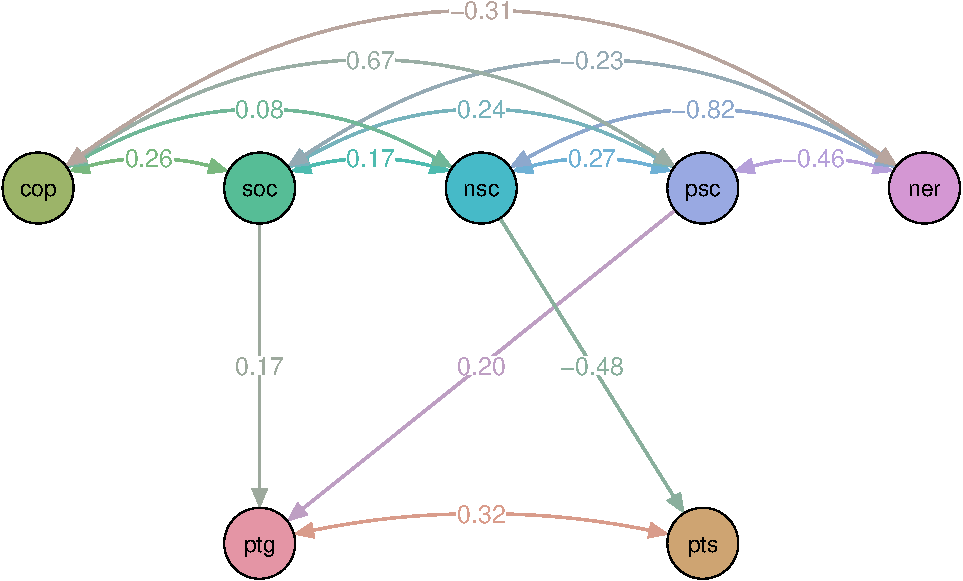
\includegraphics{self_compassion_files/figure-latex/semplot-1.pdf}
\caption{\label{fig:semplot}Direct effects of self-compassion to post-traumatic growth (\texttt{ptg}) and PTST (\texttt{pts}). \texttt{cop} = coping, \texttt{soc} = perceived social support, \texttt{nsc} = negative self compassion, \texttt{psc} = positive self compassion, \texttt{ner} = nevroticism.}
\end{figure}

The fifth model (M3) attempted to improve on the structure of M2 by adding the direct paths between neuroticism and the two outcome variables.
A comparison of the model M3 with the model M2 indicated that the model M3 did not improve fit, \(\Delta \chi^2\)(2) = 0.94, \(p =\) 0.62, with the following fit indices: \(\chi^2\)(167) = 617.86, \(\chi^2\)/df = 3.70, CFI = 0.95, NFI = 0.93, TLI = 0.93, RMSEA = 0.06, and SRMS = 0.06.
The structural component of model M3 is presented in Figure \ref{fig:semplot} (only the statistical significant path coefficients that the \(\alpha\) = 0.5 level are shown).

Having obtained a model with a good fit to the data, with the following models we tested additional specific substantive questions.
Model 4 removed from model M3 only the direct paths of the negative component of self-compassion.
This modification produced a significant decrease of fit, \(\Delta \chi^2\)(2) = 19.69, \(p =\) 0.00.
Model 5 removed from model M3 only the direct paths of the positive component of self-compassion.
Also this change produced a significant decrease of fit, \(\Delta \chi^2\)(2) = 7.07, \(p =\) 0.03.

We then considered a different also considered a mediation model (M6) with coping, perceived social support, and neuroticism as endogeneous variable, the positive and negative components of self compassion as mediator variables, and post-traumatic growth and post-traumatic stress disorder as endogeneous variables.
The fit of model M6 was very good with the following indices: \(\chi^2\)(168) = 618.00, \(\chi^2\)/df = 3.68, CFI = 0.95, NFI = 0.93, TLI = 0.93, RMSEA = 0.06, and SRMS = 0.06.
The structural component of model M6 is presented in Figure \ref{fig:mediation-model} (only the statistical significant path coefficients at the \(\alpha\) = 0.5 level are shown).

\begin{figure}
\centering
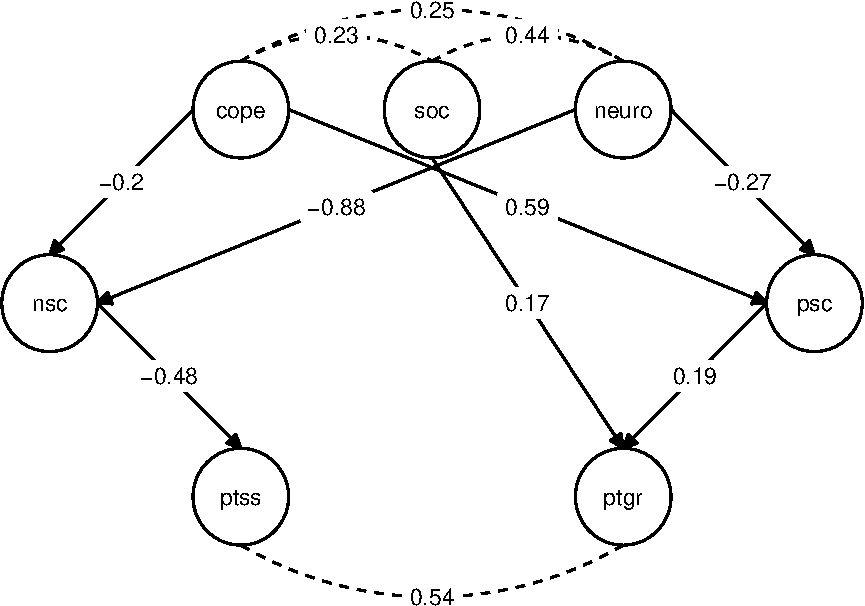
\includegraphics{self_compassion_files/figure-latex/mediation-model-1.pdf}
\caption{\label{fig:mediation-model}Structural component of a SEM model with the positive and negative components of self-compassion as mediators between coping, perceived social support, and neuroticism, as exogeneous variables, and post-traumatic growth (\texttt{ptg}) and PTST (\texttt{pts}), as endogeneous variables. \texttt{cop} = coping, \texttt{soc} = perceived social support, \texttt{nsc} = negative self compassion, \texttt{psc} = positive self compassion, \texttt{ner} = nevroticism.}
\end{figure}

Model M7 was identical to model M6, except that self-compassion was considered as a single latent variable.
The fact that we did not distinguish between the positive and negative components of self-compassion produced a significant decrease of fit, \(\Delta \chi^2\)(5) = 640.96, \(p =\) 0.00.

In a further model comparison, we considered the model M8, which is identical to model M6, except that neuroticism is used as a mediating variable, together with the two components of self-compassion, instead of being an exogenous variable.
The fit of model M8 was very bad and statistically significantly worse than the fit of model M6, \(\Delta \chi^2\)(2) = 2,010.70, \(p =\) 0.
We take this as indicating that neuroticism is unlikely to play the role of a mediating variable, together with the two components of self compassion, between the variables presently considered.

We compared models M3 and M6 with the Vuong closeness test, which indicated that they were too close too be distinguished, \(p\) = 0.74.
However, the confidence intervals for the difference in the models' AIC and BIC statistics showed an advantage for the mediation model M6: 95\% C.I.
of AIC difference = (0.14, 3.60) and 95\% C.I.
of BIC difference = (4.73, 8.19).

In order to examine the mediation structure, we compute the bias-corrected bootstrapped confidence interval with 10,000 samples.
Such approach does not rely on distribution assumptions and can be used when the assumptions of large sample size and multivariate normality may not hold (Ryu and Cheong, 2017).
If the confidence intervals do not include zero, then the null hypothesis is rejected, and the mediation effect is non-zero.

\begin{table}

\caption{\label{tab:mediation-tab}Indirect and total effects for the three endogeneous variables Coping (coping), Perceived social support (soc. supp.), and Neuroticism (neuro.) on post traumatic stress (PTSS) and post traumatic growth (PTG). S.E. = standard error; `C.I. lower` and `C.I. upper` = lower and upper limits of the 95\% bootstrap confidence interval.}
\centering
\begin{tabular}[t]{lrrrr}
\toprule
Effect & Estimate & S.E. & C.I. lower & C.I. upper\\
\midrule
Ind. eff. coping -> PTSS & 0.098 & 0.061 & -0.026 & 0.219\\
Ind. eff. coping -> PTG & 0.140 & 0.060 & 0.022 & 0.264\\
Tot. eff. coping -> PTSS & 0.195 & 0.066 & 0.072 & 0.333\\
Tot. eff. coping -> PTG & 0.238 & 0.058 & 0.127 & 0.355\\
Ind. eff. soc. supp. -> PTSS & -0.009 & 0.023 & -0.057 & 0.037\\
\addlinespace
Ind. eff. soc. supp. -> PTG & 0.003 & 0.013 & -0.023 & 0.031\\
Tot. eff. soc. supp. -> PTSS & 0.054 & 0.058 & -0.062 & 0.166\\
Tot. eff. soc. supp. -> PTG & 0.181 & 0.051 & 0.085 & 0.282\\
Ind. eff. neuro. -> PTSS & 0.505 & 0.120 & 0.283 & 0.755\\
Ind. eff. neuro. -> PTG & 0.032 & 0.103 & -0.184 & 0.232\\
\addlinespace
Tot. eff. neuro. -> PTSS & 0.571 & 0.066 & 0.451 & 0.711\\
Tot. eff. neuro. -> PTG & 0.147 & 0.052 & 0.048 & 0.252\\
\bottomrule
\end{tabular}
\end{table}

We found no (statistically significant) direct effect of coping on PTSS nor on PTG.
Conversely, we found evidence of an indirect effect of coping on PTG, with a total effect of 0.238, 95\% CI = {[}0.127, 0.355{]}.
This suggests a fully mediated effect of coping on PTG.
Instead, there was no strong evidence of a mediated effect of coping on PTSS because the confidence interval for the indirect effect included zero, 95\% CI = {[}-0.026, 0.219{]}.

There was no clear evidence of a direct effect of perceived social support on PTSS, nor evidence of an indirect effect, 95\% CI = {[}-0.057, 0.037{]}.
Instead, we found evidence of a direct effect of perceived social support on PTG, nor evidence of an indirect effect, 95\% CI = {[}-0.023, 0.031{]}.
Although the 95\% CI of the total effect did not include zero {[}0.085, 0.282{]}, it is difficult to interpret.

Finally, we found no clear evidence of a direct effect of neuroticism on PTSS, but we found evidence of an indirect effect, 95\% CI = {[}0.283, 0.755{]}, with a total effect of 0.571, 95\% CI = {[}0.451, 0.711{]}.
This suggests that the effect of neuroticism on PTSS is fully mediated.
Conversely, we found no clear evidence of a direct effect of neuroticism on PTG, nor evidence of an indirect effect of neuroticism on PTG, with a total effect of 0.032, 95\% CI = {[}-0.184, 0.232{]}.

\hypertarget{discussion}{%
\section{Discussion}\label{discussion}}

Main points.

for a recent development, see also Gu et al. (2020)

\begin{itemize}
\item
  We found evidence that a model with a single component of SC is inadequate, whereas a model which distinguishes the positive and negative component of SC is more adequate to account for the data.
\item
  We found evidence of a better fit for a model which adds the positive component of SC to a model with only the negative component of SC.
\item
  Consistently with (ref), we found evidence that SC is better understood as a mediation variable.
\item
  We found evidence that a model which include nevroticism is more adequate than a model with only SC.
\end{itemize}

In conclusion, we found not evidence that the construct of SC can be subsumed by the constructs of negative affect and nevroticism.
Instead, we found evidence, consistently with (ref), that SC plays a mediating role between coping, perceived social support, and nevroticism, on the one side, and PTSS and PTG, on the other.
Importantly, we also found that nevroticism and SC are both important in accounting for PTSS and PTG -- in other words, we cannot reduce SC to nevroticism.
Instead, our data suggest that the two components of SC and nevroticism play a different structural role in a nomological network having PTSS and PTG as endogenous variables.

\newpage

\hypertarget{references}{%
\section{References}\label{references}}

\begingroup
\setlength{\parindent}{-0.5in}
\setlength{\leftskip}{0.5in}

\hypertarget{refs}{}
\begin{CSLReferences}{1}{0}
\leavevmode\hypertarget{ref-bandalos2014relative}{}%
Bandalos, D. L. (2014). Relative performance of categorical diagonally weighted least squares and robust maximum likelihood estimation. \emph{Structural Equation Modeling: A Multidisciplinary Journal}, \emph{21}(1), 102--116.

\leavevmode\hypertarget{ref-geiger2018self}{}%
Geiger, M., Pfattheicher, S., Hartung, J., Weiss, S., Schindler, S., Wilhelm, O., \& Kandler, C. (2018). Self--compassion as a facet of neuroticism? A reply to the comments of {Neff, T{ó}Th--Kir{á}Ly, and Colosimo (2018)}. \emph{European Journal of Personality}, \emph{32}(4), 393--404.

\leavevmode\hypertarget{ref-gu2020development}{}%
Gu, J., Baer, R., Cavanagh, K., Kuyken, W., \& Strauss, C. (2020). Development and psychometric properties of the sussex-oxford compassion scales (SOCS). \emph{Assessment}, \emph{27}(1), 3--20.

\leavevmode\hypertarget{ref-gu2020development}{}%
Gu, J., Baer, R., Cavanagh, K., Kuyken, W., \& Strauss, C. (2020). Development and psychometric properties of the sussex-oxford compassion scales (SOCS). \emph{Assessment}, \emph{27}(1), 3--20.

\leavevmode\hypertarget{ref-kandler2017old}{}%
Kandler, C., Pfattheicher, S., Geiger, M., Hartung, J., Weiss, S., \& Schindler, S. (2017). Old wine in new bottles? The case of self--compassion and neuroticism. \emph{European Journal of Personality}, \emph{31}(2), 160--169.

\leavevmode\hypertarget{ref-little2013longitudinal}{}%
Little, T. D. (2013). \emph{Longitudinal structural equation modeling}. Guilford press.

\leavevmode\hypertarget{ref-montero2018self}{}%
Montero-Marin, J., Kuyken, W., Crane, C., Gu, J., Baer, R., Al-Awamleh, A. A., Akutsu, S., Araya-Véliz, C., Ghorbani, N., Chen, Z. J., \& others. (2018). Self-compassion and cultural values: A cross-cultural study of self-compassion using a multitrait-multimethod (MTMM) analytical procedure. \emph{Frontiers in Psychology}, \emph{9}, 2638.

\leavevmode\hypertarget{ref-muris2016protective}{}%
Muris, P. (2016). A protective factor against mental health problems in youths? A critical note on the assessment of self-compassion. \emph{Journal of Child and Family Studies}, \emph{25}(5), 1461--1465.

\leavevmode\hypertarget{ref-muris2018good}{}%
Muris, P., Broek, M. van den, Otgaar, H., Oudenhoven, I., \& Lennartz, J. (2018). Good and bad sides of self-compassion: A face validity check of the self-compassion scale and an investigation of its relations to coping and emotional symptoms in non-clinical adolescents. \emph{Journal of Child and Family Studies}, \emph{27}(8), 2411--2421.

\leavevmode\hypertarget{ref-muris2020process}{}%
Muris, P., \& Otgaar, H. (2020). The process of science: A critical evaluation of more than 15 years of research on self-compassion with the self-compassion scale. \emph{Mindfulness}, \emph{11}(6), 1469--1482.

\leavevmode\hypertarget{ref-muris2016protection}{}%
Muris, P., Otgaar, H., \& Petrocchi, N. (2016). Protection as the mirror image of psychopathology: Further critical notes on the self-compassion scale. \emph{Mindfulness}, \emph{7}(3), 787--790.

\leavevmode\hypertarget{ref-muris2019stripping}{}%
Muris, P., Otgaar, H., \& Pfattheicher, S. (2019). Stripping the forest from the rotten trees: Compassionate self-responding is a way of coping, but reduced uncompassionate self-responding mainly reflects psychopathology. \emph{Mindfulness}, \emph{10}(1), 196--199.

\leavevmode\hypertarget{ref-muris2019stripping}{}%
Muris, P., Otgaar, H., \& Pfattheicher, S. (2019). Stripping the forest from the rotten trees: Compassionate self-responding is a way of coping, but reduced uncompassionate self-responding mainly reflects psychopathology. \emph{Mindfulness}, \emph{10}(1), 196--199.

\leavevmode\hypertarget{ref-muris2017protection}{}%
Muris, P., \& Petrocchi, N. (2017). Protection or vulnerability? A meta-analysis of the relations between the positive and negative components of self-compassion and psychopathology. \emph{Clinical Psychology \& Psychotherapy}, \emph{24}(2), 373--383.

\leavevmode\hypertarget{ref-muthen2017mplus}{}%
Muthén, L., \& Muthén, B. (2017). Mplus. \emph{Statistical Analysis with Latent Variables. User's Guide}, \emph{8}.

\leavevmode\hypertarget{ref-neff2003self}{}%
Neff, K. D. (2003a). Self-compassion: An alternative conceptualization of a healthy attitude toward oneself. \emph{Self and Identity}, \emph{2}(2), 85--101.

\leavevmode\hypertarget{ref-neff2003development}{}%
Neff, K. D. (2003b). The development and validation of a scale to measure self-compassion. \emph{Self and Identity}, \emph{2}(3), 223--250.

\leavevmode\hypertarget{ref-neff2019examining}{}%
Neff, K. D., Tóth-Király, I., Yarnell, L. M., Arimitsu, K., Castilho, P., Ghorbani, N., Guo, H. X., Hirsch, J. K., Hupfeld, J., Hutz, C. S., \& others. (2019). Examining the factor structure of the self-compassion scale in 20 diverse samples: Support for use of a total score and six subscale scores. \emph{Psychological Assessment}, \emph{31}(1), 27--45.

\leavevmode\hypertarget{ref-neff2019examining}{}%
Neff, K. D., Tóth-Király, I., Yarnell, L. M., Arimitsu, K., Castilho, P., Ghorbani, N., Guo, H. X., Hirsch, J. K., Hupfeld, J., Hutz, C. S., \& others. (2019). Examining the factor structure of the self-compassion scale in 20 diverse samples: Support for use of a total score and six subscale scores. \emph{Psychological Assessment}, \emph{31}(1), 27--45.

\leavevmode\hypertarget{ref-seppala2017oxford}{}%
Seppälä, E. M., Simon-Thomas, E., Brown, S. L., Worline, M. C., Cameron, C. D., \& Doty, J. R. (2017). \emph{The oxford handbook of compassion science}. Oxford University Press.

\leavevmode\hypertarget{ref-strauss2016compassion}{}%
Strauss, C., Taylor, B. L., Gu, J., Kuyken, W., Baer, R., Jones, F., \& Cavanagh, K. (2016). What is compassion and how can we measure it? A review of definitions and measures. \emph{Clinical Psychology Review}, \emph{47}, 15--27.

\leavevmode\hypertarget{ref-wadsworth2018examining}{}%
Wadsworth, L. P., Forgeard, M., Hsu, K. J., Kertz, S., Treadway, M., \& Björgvinsson, T. (2018). Examining the role of repetitive negative thinking in relations between positive and negative aspects of self-compassion and symptom improvement during intensive treatment. \emph{Cognitive Therapy and Research}, \emph{42}(3), 236--249.

\end{CSLReferences}

\endgroup

\renewcommand{\appendixname}{Supplementary Information}


\clearpage
\makeatletter
\efloat@restorefloats
\makeatother


\begin{appendix}
\section{}
Some general data properties, which are needed to determine the most
appropriate analytical approach, were examined. The absence of
multivariate normality in all items (Mardia's Test: sig. \textless{}
.01), and missing data (11.3\% of the cases, with a completely random
distribu- tion of the missing data; Little's test sig. p \textgreater{}
.05) were observed. Given the ordinal nature of the data, the weighted
least square with adjusted mean and variance (WLSMV) (Beauducel \&
Herzberg, 2006; Rhemtulla et al., 2012) approach was used as an
estimation method of the factor models.

In all studied models, goodness of fit was determined by using the
comparative fit index (CFI), the Tucker- Lewis index (TLI) and the root
mean square of approxi- mation (RMSEA). For the CFI and TLI, values
above .90 and .95, respectively, indicate an acceptable and adequate fit
(Chen, 2007, Hu \& Bentler, 1999). In the case of the RMSEA, values
below .08 and .05, respectively, indicate an acceptable and appropriate
fit (Cheung \& Rensvold, 2002). To determine the significance of the fit
differences between the nested or equivalent models, Chen (Chen, 2007)
and Cheung and Resvold's (Cheung \& Rensvold, 2002) recommendations were
followed. According to these scholars, increases in the CFI and TLI less
than .01 and decreases in the RMSEA less than .015 suggest that there
are no substantial differences in fit among the com- pared models. All
analyses were performed by using MPlus v 7.3 (Muthén \& Muthén, 2014).

The following data analytic strategy was adopted. First, six measurement
models were estimated via ICM-CFA (independent clusters model of
confirmatory factor analysis). Second, and based on the results from the
previous step, an ESEM model with a similar configuration to the
four-correlated-factor structure proposed by the DSM--5 was estimated.
Third, an ESEM bifactor model was estimated to explore the existence of
a common source of variance to all PTSD symptoms. To estimate the
model-based reliability for each factor the omega index was calculated
in the case of the first order models (McDonald, 1999). The omega
hierarchical index (Zinbarg et al., 2006) and the omega sub-scale were
estimated in the case of the bifactor model (Reise, 2012). These indexes
quantify the degree to which the factor scores accurately reflect the
position of the subject in the latent variable (values above .70 are
required to ensure the psychometric interpretability of the factor). To
estimate the internal consistency of each factor, Cronbach's alpha was
used.

\begin{figure}
\centering
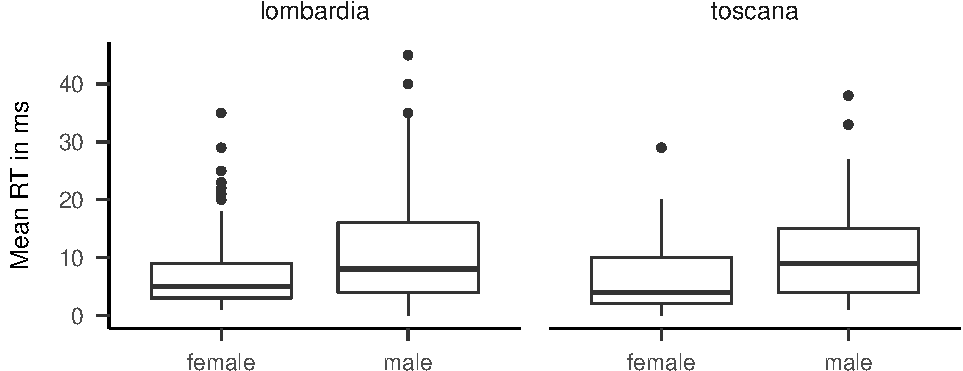
\includegraphics{self_compassion_files/figure-latex/unnamed-chunk-23-1.pdf}
\caption{\label{fig:unnamed-chunk-23}Boxplots of mean response times for all
fast tasks, split by age groups. See Table 1 for an explanation of the
task names.}
\end{figure}
\end{appendix}

\end{document}
